\begin{center}

\begin{tikzpicture}
    \begin{scope}[x={(current page.south east)},y={(current page.north west)}]
        \node[anchor=south west,inner sep=0, ] (image)  at (0.55, 0.35) {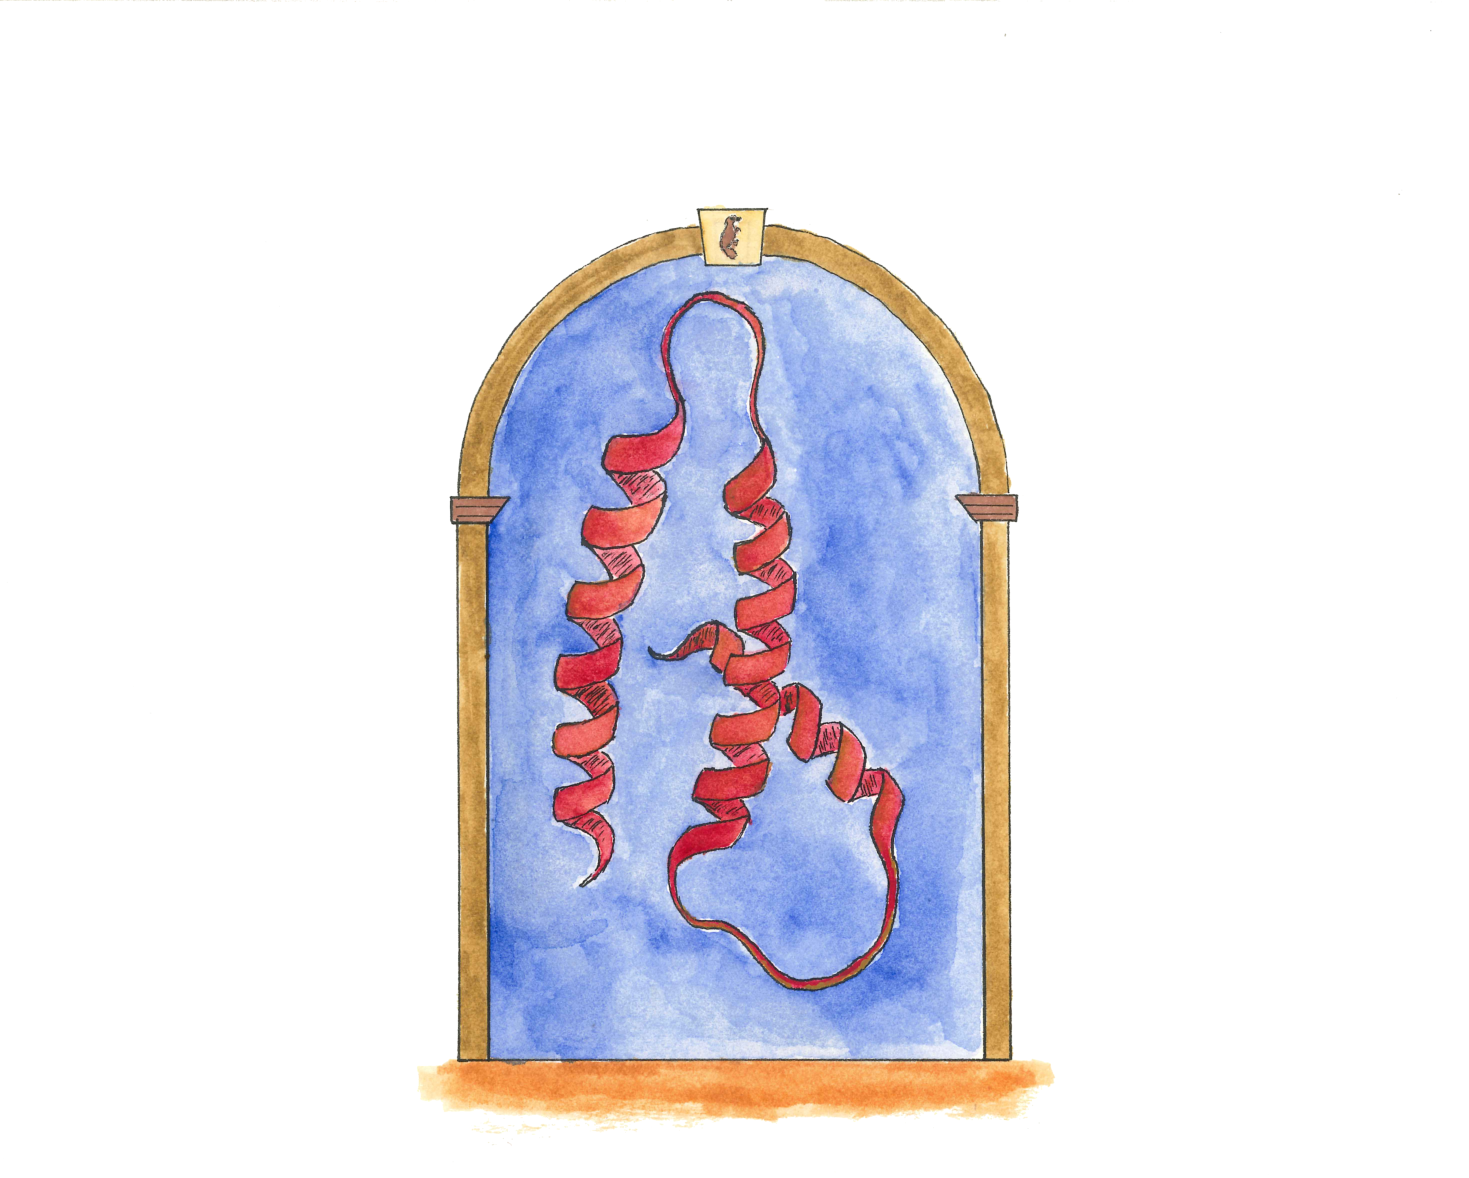
\includegraphics[trim={7cm, 0, 7cm, 0}, clip, height=0.55\pageheight]{scans/inner_cover.pdf}};
    	\if\helplines1
        	\draw[help lines,xstep=.1,ystep=.1] (0,0) grid (\N,\N);
        \fi
        \if\helplines0
        	\path[help lines,xstep=.1,ystep=.1] (0,0) grid (\N,\N);
        \fi
        
        \node[align=center, anchor=north] (en) at (0.3, 0.8) {\english{\Large Explanation of the cover}};
        
        \node[align=justify, anchor=north, below=1cm of en, text width=0.4\pagewidth] {\english{The cover depicts a protein structure under an arch, a punny reference between protein structures, and the importance of the structure of the data in deep learning. This is, incidentally, why some people call it \emph{structured learning}. The arch style is inspired by the works of Vitruvius, a throwback to the Reinessance, which matches the style of the interior of the thesis.
        
        \vspace{0.5em}
        
        \doindent The keystone depicts a tiny rampant platypus.}};
        
        \node[align=left, anchor=west] (es) at (0.1, 0.3)  {\spanish{\Large Explicación de la portada.}};
        
        
        \node[align=justify, anchor=west, text width=0.8\pagewidth] (es) at (0.1, 0.18)  {\spanish{La portada muestra la estructura de una proteína bajo un arco, un juego de palabras entre las estructuras de proteínas, y la importancia de la estructura de los datos en aprendizaje profundo. Por esta razón algunos autores lo llaman \emph{aprendizaje estructurado}.
        El estilo del arco está inspirado por los diseños de Vitruvio, una referencia al Renacimiento, que harmoniza con el estilo del interior de la tésis.
        
                \vspace{0.5em}
                
        \doindent La clave representa un ornitorrinco rampante.}};
        
    \end{scope}
\end{tikzpicture}
\end{center}
